% !TeX spellcheck = en_UK

\section{3C295 and the Extended Groth Strip}\label{section.3c295+EGS}
\pg
In this section, we describe the work done as part of this PhD on calibrating and imaging interferometric data on the Extended Groth Strip, an extragalactic field with rich multi-wavelength coverage. This work can be described in two parts: first, we created a high-resolution, multi-wavelength model of a bright, diffuse source near the field, 3C295. This source lies at coordinates . Only with this model could work on the Extended Groth Strip proper begin: without the model, the noise in the image would be dominated by artefacts rather than thermal noise, and so sensitivity would not increase with additional data. 

\pg
This section is thus logically split into two separate parts. First, we discuss obtaining a high-resolution, multi-wavelength model for 3C295. Then, we show the work done investigating whether direction-dependent effects were strong enough to require a multi-facet calibration of the Extended Groth Strip.


\subsection{Modelling a calibrator source: 3C295}\label{section.3c295}

\pg
Let us begin by describing the method used to acquire a high-quality, high-resolution multi-wavelength model of 3C295. 

\subsubsection{Initial Model}
\pg
The initial model was acquired from the NASA/IPAC Extragalactic Database\footnote{\hyperref[here]{https://ned.ipac.caltech.edu/}}. Because no high-resolution models exist for 3C295 at our observing frequencies, which span quite a large bandwidth, care must be taken not to bias our model in an unphysical direction. We therefore perform self-calibration loops\footnote{see [TODO; ADD REFERENCE]} rounds in various subbands, since we have no \emph{a priori} knowledge of the spectral behaviour of the source as a whole.

\pg
We thus begin each self-calibration loop with a very simple sky model: we assume that 3C295 is dominated by two point sources, located at the emission peaks of a VLA observation made at an appropriate resolution , $0.2''$ \citep[see][]{1991AJ....101.1623P}. The image is shown in Fig. \ref{fig.vla.3c295}. By self-calibrating within various intervals of our overall bandwidth, we expect to be able to recover source structure without undue bias. 

\begin{figure}[h!]
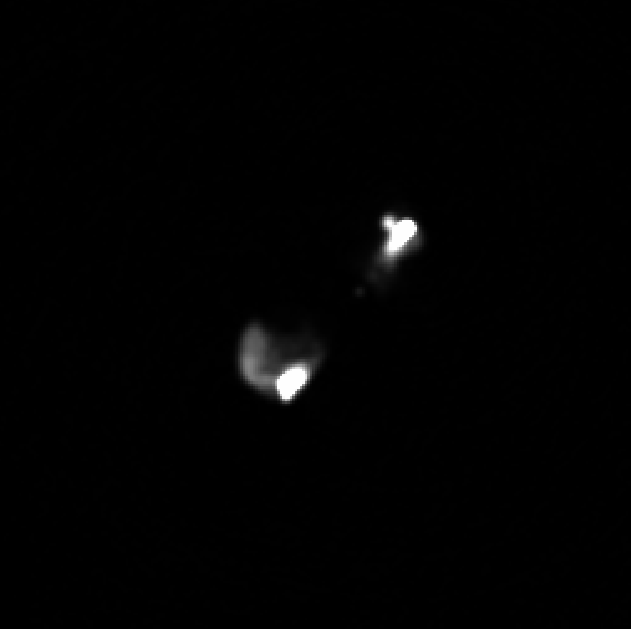
\includegraphics[width=0.5\linewidth]{images/3c295-vla}
\caption{\label{fig.vla.3c295}VLA observation of 3C295. Pixel size is $0.2''$.}
\end{figure}

\pg
PyBDSM \citep{2015ascl.soft02007M} was used to extract this two-point model. The first check was to see whether the two-point model converges, within multiple rounds of self-cal, towards the same result as when the same data is calibrated with an outside, high-resolution sky model. Standard practice is to begin with a $uv$-cut excluding the shorter baselines, so that the start of the self-calibration is dominated by compact emission. This allows the procedure to converge more quickly. For this reason, each calibration step in the self-calibration loop is made with a $uv$-cut excluding only baselines shorter than 100 meters (essentially excluding the core LOFAR stations). This is because we wish to begin by only keeping the longer baselines, but too strict a $uv$-cut results in under-constrained calibration solutions. Amplitude and phase are both solved for and applied. Since imaging does not have this restriction, imaging is performed with a $uv$-cut excluding all baselines shorter than 100km. 

\pg
We begin by testing the self-calibration convergence on a single LOFAR subband, SB030 (centred at 117.61 MHz, bandwidth of 200 kHz). The self-calibration, excluding core LOFAR stations for calibration and short baselines for imaging, converges towards decreased artefacts and noise in the field. This can be seen in Fig. \ref{fig.residuals.3c295.selfcal.uvcut}, which shows the residual image as a function of self-calibration. 

\begin{figure*}[t!]
\centering
\begin{subfigure}{.43\textwidth}
\resizebox{\hsize}{!}{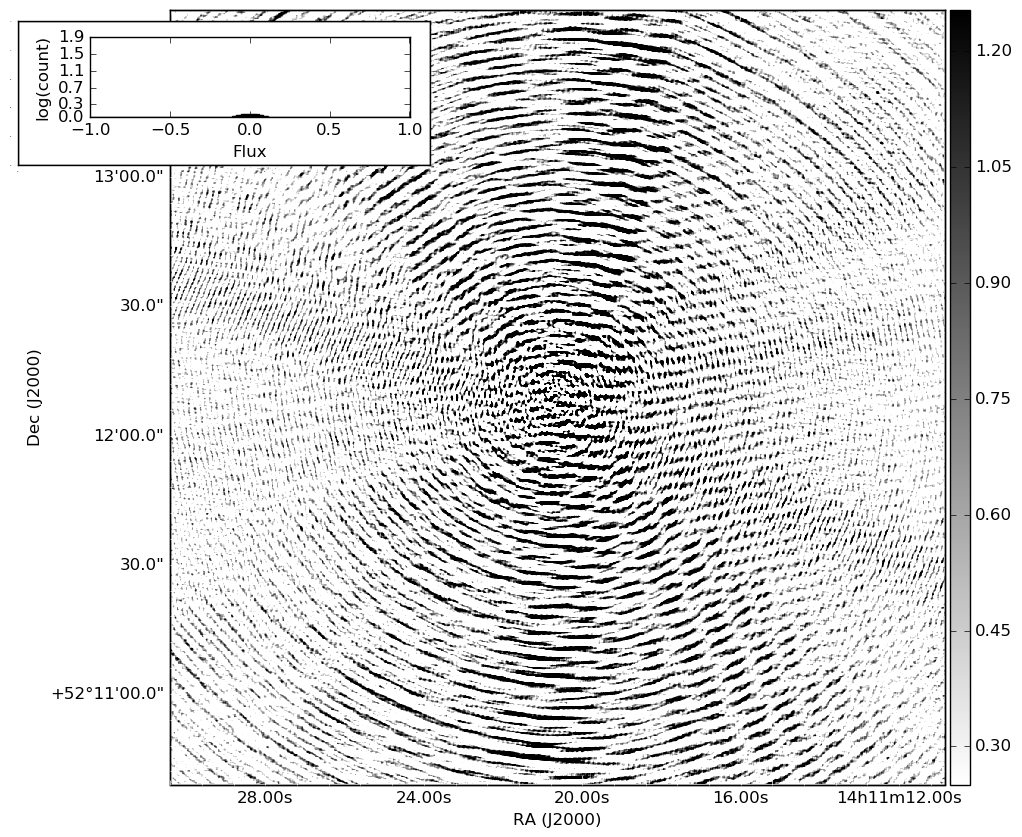
\includegraphics{images/3c295-sb030-uvcut-SC1.png}}
\caption{\label{fig.residuals.3c295.selfcal.uvcut.SC1}First pass of self-calibration: many artefacts present.}
\end{subfigure}
\hfill
\begin{subfigure}{.43\textwidth}
\resizebox{\hsize}{!}{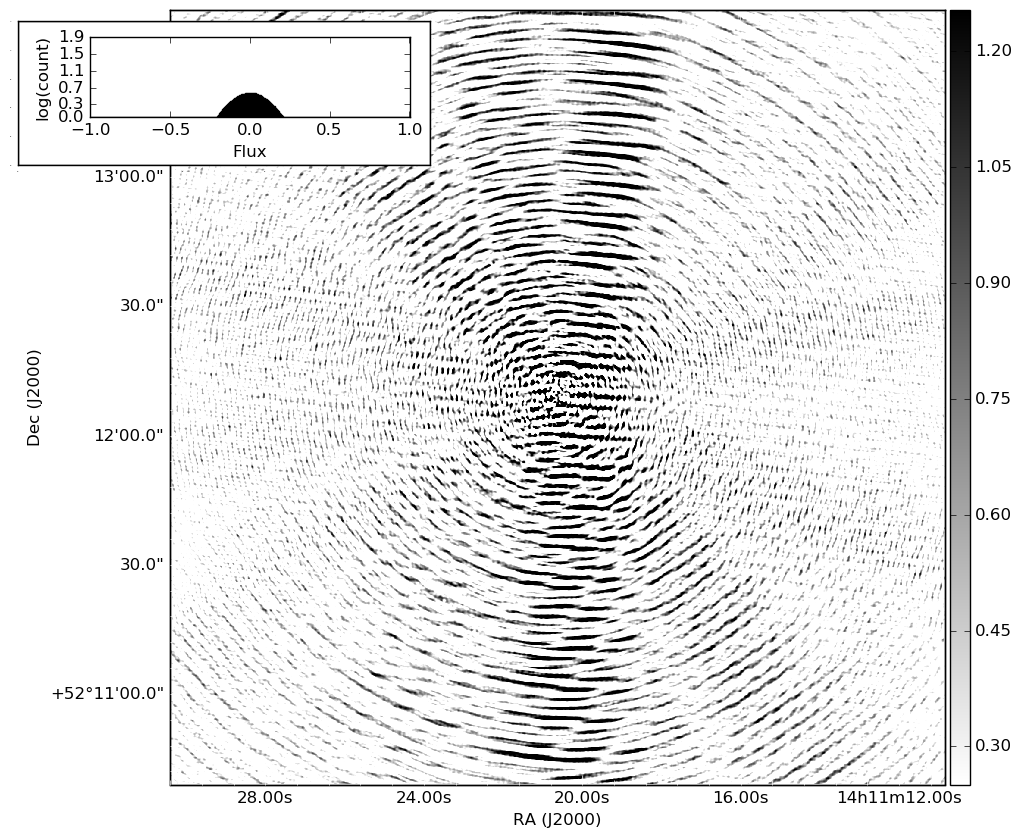
\includegraphics{images/3c295-sb030-uvcut-SC3.png}}
\caption{\label{fig.residuals.3c295.selfcal.uvcut.SC3} Third pass of self-calibration: decreased artefacts but still a ways to go.}
\end{subfigure}
\hfill
\begin{subfigure}{.43\textwidth}
\resizebox{\hsize}{!}{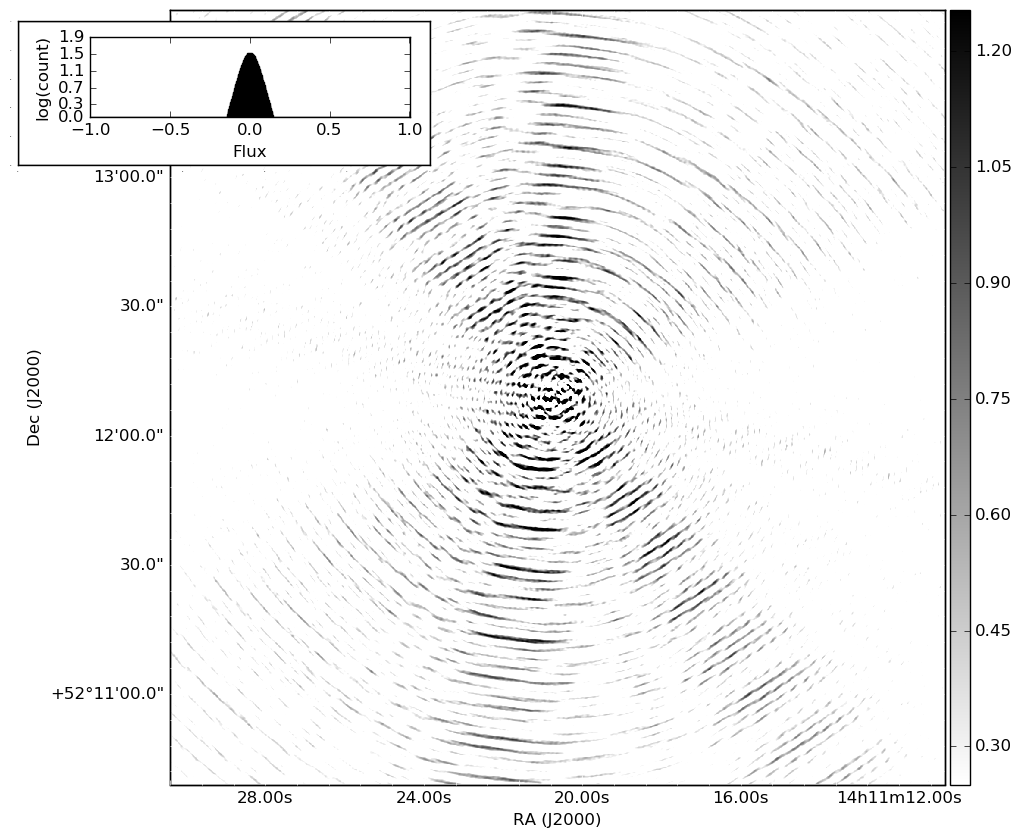
\includegraphics{images/3c295-sb030-uvcut-SC6.png}}
\caption{\label{fig.residuals.3c295.selfcal.uvcut.SC6} Sixth pass: significant improvement over Fig. \ref{fig.residuals.3c295.selfcal.uvcut.SC1}.}
\end{subfigure}
\hfill
\begin{subfigure}{.43\textwidth}
\resizebox{\hsize}{!}{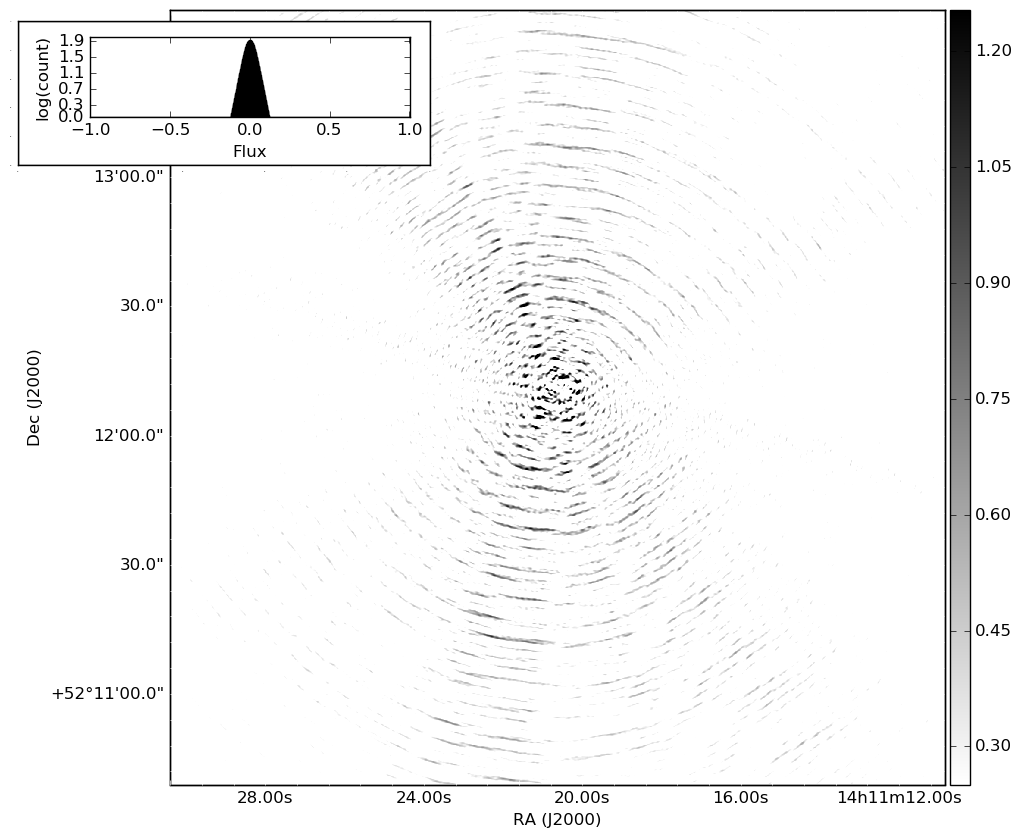
\includegraphics{images/3c295-sb030-uvcut-SC9.png}}
\caption{\label{fig.residuals.3c295.selfcal.uvcut.SC9} Ninth pass. Some artefacts remain, so self-calibration could be taken further.}
\end{subfigure}
\caption{\label{fig.residuals.3c295.selfcal.uvcut} Residual images of 3C295 over various rounds of self-calibration. We see that artefacts in the field decrease as more passes are completed, and that the pixel distribution becomes more and more peaked around zero: noise decreases in the image along with artefacts.}

\end{figure*}

\pg
For each round of self-calibration, a custom mask image is made with the restored image from the previous: this mask is equal to 1 for all pixels with a value above a $\sigma$-threshold of 5, and zero elsewhere. Then, this mask is inspected: all points which are likely artefacts (i.e. away from the source) are flagged off from the mask. This allows the mask to "naturally" expand over iterations. In so doing, we obtain the model shown in Fig. \ref{fig.restored.3c295.VLAmodel.selfcal.uvcut.SC9.normalised} after a total of 9 self-calibration passes. We compare this result to an external high-resolution model made at a similar frequency (SB090 - centred on 128.33 MHz, bandwidth 200 kHz - of the same dataset). Note that the pixel values in both Fig. \ref{fig.restored.3c295.VLAmodel.selfcal.uvcut.SC9.normalised} and \ref{fig.restored.3c295.externalmodel.selfcal.uvcut.SC12.normalised} have been normalised, since neither model is boot-strapped\footnote{Boot-strapping is the practice of forcing the flux scale of an image by ensuring that a well-known, well-studied object with reliably-known flux at this frequency has the expected value in the image.} at this point.

\begin{figure*}[t!]
\centering
\begin{subfigure}{.43\textwidth}
\resizebox{\hsize}{!}{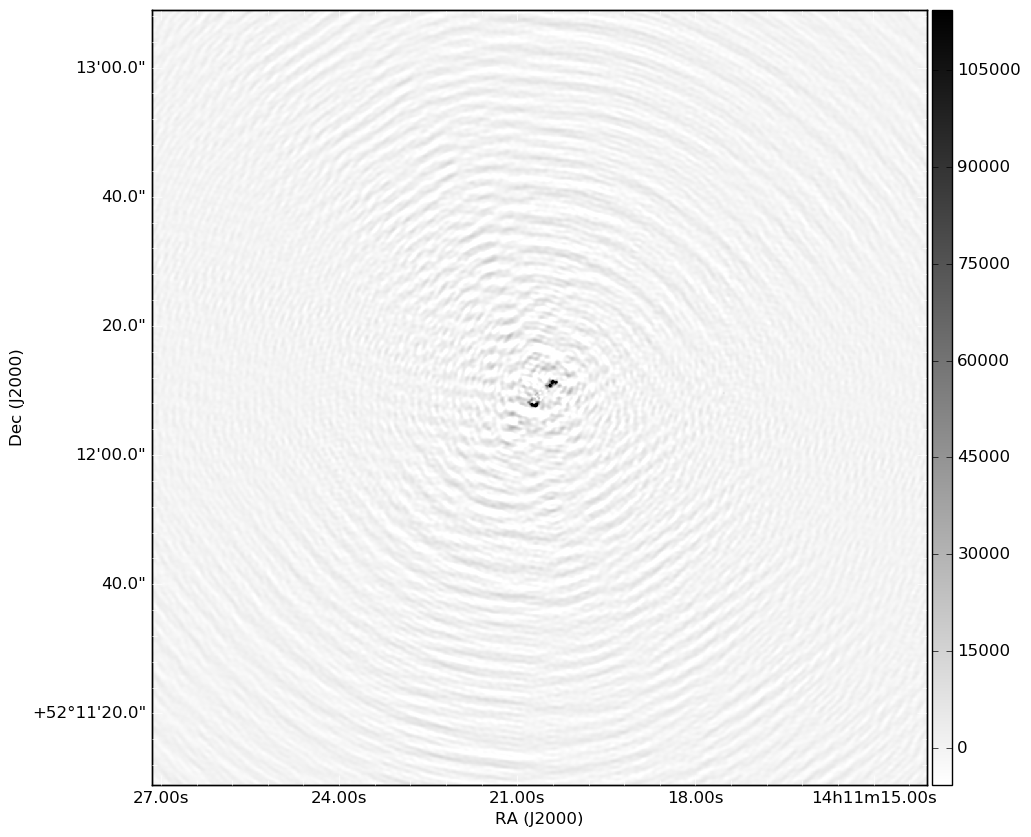
\includegraphics{images/3c295-vla-model-SC9-uvcut-normalised.png}}
\caption{\label{fig.restored.3c295.VLAmodel.selfcal.uvcut.SC9.normalised} 9th pass of self-cal, starting from the 2-point model extracted Fig. \ref{fig.vla.3c295}.}
\end{subfigure}
\hfill
\begin{subfigure}{.43\textwidth}
\resizebox{\hsize}{!}{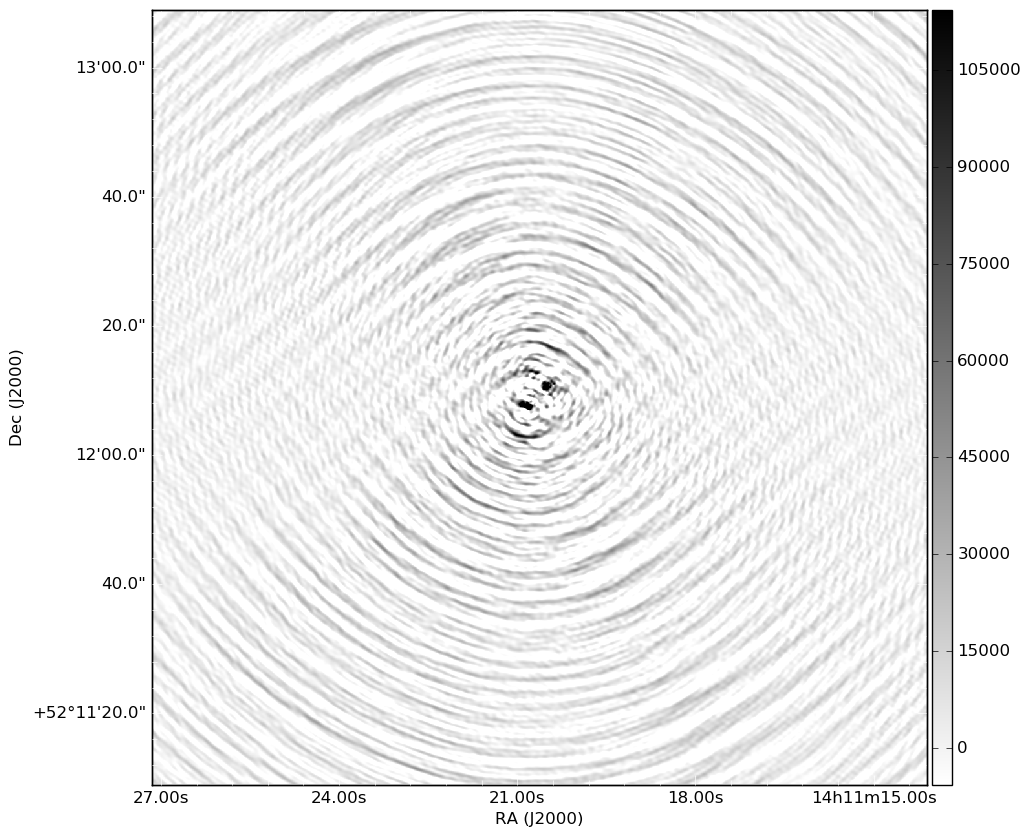
\includegraphics{images/3c295-sb90-model-pass12-uvcut-normalised.png}}
\caption{\label{fig.restored.3c295.externalmodel.selfcal.uvcut.SC12.normalised} Same data calibrated using an external model provided by Cyril Tasse..}
\end{subfigure}
\caption{\label{fig.restored.comparison.externalSC12.vlaSC9} Both of these images were made with a $uv$-cut flagging all baselines shorter than 100km. We see that both models give similar positions and shapes for the hotspots, though Fig. \ref{fig.restored.3c295.VLAmodel.selfcal.uvcut.SC9.normalised} has less artefacts than Fig. \ref{fig.restored.3c295.externalmodel.selfcal.uvcut.SC12.normalised}. Flux scale is normalised in both images.}
\end{figure*}

\newpage





%
%
%\newpage
%\subsection{The Boötes field}\label{subsection.EGS}
%
%\pg
%The Extended Groth Strip (henceforth, EGS) is one of the so-called ``famous extragalactic fields". has been long observed as part of the All-Wavelength Extended Groth Strip International Survey collaboration (\citepads{2007ApJ...660L...1D}), which later became part of the CANDELS collaboration (\citepads{2011ApJS..197...35G}). The field is centred at $\alpha=14^h17^m,\delta=+52\deg 30'$, placing it between the tail of Ursa Major and Draco. The $\lambda$-coverage is summarised in \cref{bootes-coverage-table}, and the associated pointings given in \cref{bootes-coverage-image}
%
%%\newpage
%
%\begin{table}[h!]
%\centering
%\caption{Multi-wavelength coverage of the Boötes field}
%\label{bootes-coverage-table}
%\begin{tabular}{|ccccc|} \hline
%Catalog                    & $\lambda$,$\nu$,band           & Sensitivity              & Resolution               & Source                            \\\hline\hline
%XBootes                    & 0.5-0.7 keV                    & $4(8).10^{-15}$ ergs cm$^{-2}\text{s}^{-1}$ & 0.492''                & \citepads{2005ApJS..161....1M}    \\\hline
%\multirow{6}{*}{NOAO-Deep} & B$_\text{W}$                   & 26.6 mag                 & \multirow{6}{*}{1''\footnote{Seeing-limited. Value given at: \url{https://www.noao.edu/noao/noaodeep/DR3/optimagepropsdr3.html}}}                                              &\multirow{6}{*}{\citepads{1999ASPC..191..111J}}\\
%                           & R                              & 25.8 mag                 &                          &                                   \\
%                           & I                              & 25.5 mag                 &                          &                                   \\
%                           & J                              & 20.2 mag                 &                          &                                   \\
%                           & H                              & 19.6 mag                 &                          &                                   \\
%                           & K                              & 19.5 mag                 &                          &                                   \\\hline
%\multirow{4}{*}{WISE}      & $22\mu$m                       & 5.9 mJy                  & \multirow{4}{*}{1.375''\footnote{Value taken from the \hyperlink{http://wise2.ipac.caltech.edu/docs/release/allsky/expsup/sec1_2.html}{Executive Summary of WISE All-Sky Release Data Products}, under section I.2.a. Image Atlas}} &\multirow{4}{*}{\citepads{2012wise.rept....1C}}              \\
%                           & $12\mu$m                       & 0.73 mJy                 &                          &                                   \\
%                           & $4.6\mu$m                      & 0.1 mJy                  &                          &                                   \\
%                           & $3.4\mu$m                      & 0.048 mJy                &                          &                                   \\\hline
%WSRT                       & 1.4 GHz                        & 0.028 mJy                & 13''$\times$27''         & \citepads{2002AJ....123.1784D}    \\
%VLA                        & 324.5 MHz                      & 0.5 mJy                  & 6''                      & \citepads{2015MNRAS.450.1477C}    \\
%GMRT                       & 153 MHz                        & 5 mJy                    & 26''$\times$22''         & \citepads{2011AnA...535A..38I}    \\
%LOFAR-HBA                  & 144 MHz                        & TBA                      & 1.5''                    &   TBA                             \\\hline
%\multirow{3}{*}{LOFAR-LBA} & 62 MHz                         & 25 mJy                   & 4''                      & \multirow{3}{*}{\citepads{2014ApJ...793...82V}}    \\
%                           & 46 MHz                         & 40 mJy                   & 5''                      &                                   \\
%                           & 34 MHz                         & 60 mJy                   & 7''                      &                                   \\\hline
%\end{tabular}
%\end{table}
%
%\begin{figure}[h!]
%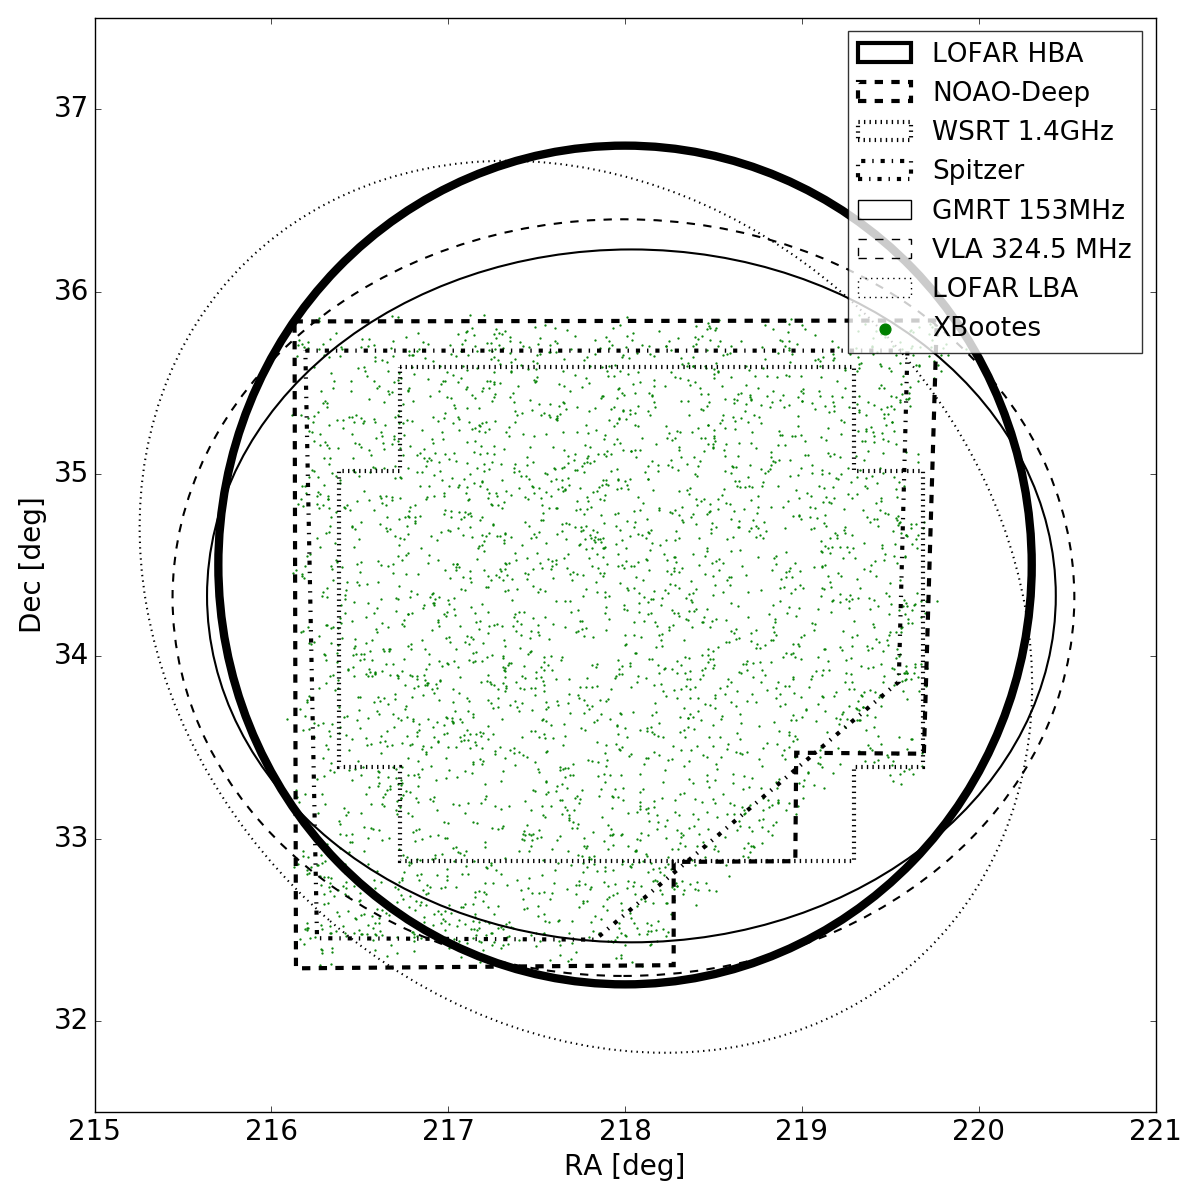
\includegraphics[width=\linewidth]{images/SkyCoverageMap}
%\caption{Sky coverage over the Boötes extragalactic field}
%\label{bootes-coverage-image}
%\end{figure}
%
%It has notably been the subject of very deep Hubble Space Telescope observations, the resolution of which VLBI with LOFAR international can now begin to match.

%
%talk about the field: location, size, history
%
%talk about multi-lambda coverage: put coverage figure here!
%
%\subsection{High-resolution imaging: calibrating the International Baselines}